\documentclass[12pt]{article}
\usepackage{amsmath}
\usepackage{graphicx}
\usepackage{natbib}
\usepackage{url}
\usepackage{blkarray}

\newcommand{\blind}{0}

\addtolength{\oddsidemargin}{-.5in}
\addtolength{\evensidemargin}{-1in}
\addtolength{\textwidth}{1in}
\addtolength{\textheight}{1.7in}
\addtolength{\topmargin}{-1in}


% For including theorem environment
\usepackage[utf8]{inputenc}
\usepackage{amsthm}
% References
\usepackage{natbib}
\setcounter{tocdepth}{2}
\setcounter{secnumdepth}{3}
\usepackage[depth=2]{bookmark}
% To add algorithms 
\usepackage[ruled,vlined]{algorithm2e}
% To edit the line spacing of different sections of the document.
\usepackage{setspace}
% To use declaremathoperator/equation references 
\usepackage{amsmath}
% Using english language
\usepackage[english]{babel}
% To include captions
\usepackage{caption}
% For labeled lists
\usepackage{enumerate}
\usepackage{enumitem}
% For multiline comments
\usepackage{comment}
% For bold symbols
\usepackage{bm}
% To automatize the environments you reference to.
\usepackage{cleveref}
% for figures
\usepackage{tikz}
% For indicator functions
\usepackage{dsfont}
% For having \bbfonts.
\usepackage{amsfonts}
% For other important symbols
\usepackage{amssymb}
% For the double-hat symbol
\usepackage{accents}
% To improve tables:
\usepackage{multirow}
% To rotate a table in a full page:
\usepackage{rotating}
% To add vertical tables.
\usepackage{pdflscape}
% To use hyperlinks to emails and papers.
\usepackage{hyperref}
%\hypersetup{
%	colorlinks=true,
%	linkcolor=red,0
%	urlcolor=blue,
%	citecolor=blue
%}
% Packages necessary for pretty plots
\usepackage{lmodern}
\usepackage{siunitx}
\usepackage{booktabs}
\usepackage{etoolbox}
\usepackage{caption}
% To display inequalities in text.
\usepackage[T1]{fontenc}

% Define the floor and ceiling operators.
\usepackage{mathtools}
\DeclarePairedDelimiter\ceil{\lceil}{\rceil}
\DeclarePairedDelimiter\floor{\lfloor}{\rfloor}

% Block matrix tool:
\newcommand{\bigzero}{\mbox{\normalfont\Large\bfseries 0}}
\newcommand{\rvline}{\hspace*{-\arraycolsep}\vline\hspace*{-\arraycolsep}}

%% Theorem/definition environments.
\newtheorem{thm}{Theorem}
\newtheorem{cor}{Corollary}
\newtheorem{ex}{Example}
\newtheorem{prop}{Proposition}
\newtheorem{lemma}{Lemma}
\newtheorem{assumption}{Assumption}

\theoremstyle{definition}
\newtheorem{definition}{Definition}
\newtheorem{remark}{Remark}

\newtheorem*{thm*}{Theorem}
\newtheorem*{cor*}{Corollary}
\newtheorem*{ex*}{Example}
\newtheorem*{prop*}{Proposition}
\newtheorem*{lemma*}{Lemma}
\newtheorem*{assumption*}{Assumption}

\theoremstyle{definition}
\newtheorem*{definition*}{Definition}
\newtheorem*{remark*}{Remark}




% Constantly used operators
\newcommand{\adj}{\mathrm{adj}}
\newcommand{\mt}{\top}

% Other useful operators
\newcommand{\norm}[2]{\left\lVert#1\right\rVert_{#2}}
\newcommand{\indv}[1]{\mathds{1}_{#1}}
\newcommand{\ind}[1]{\mathds{1}\left(#1\right)}
\newcommand{\bone}{{\mathbf{1}}}		% zero vector
\newcommand{\bzero}{{\mathbf{0}}}		% zero vector
\newcommand{\calO}{\mathcal{O}}

% Command for positive definite matrices.
\newcommand{\pdset}[1]{\cS^{#1 \times #1}_{+}}
\newcommand{\matset}[2]{\bbR^{#1 \times #2}}
\newcommand{\bhat}[1]{\widehat{#1}}
\newlength{\dhatheight}
\newcommand{\bbhat}[1]{%
	\settoheight{\dhatheight}{\ensuremath{\hat{#1}}}%
	\addtolength{\dhatheight}{-0.35ex}%
	\hat{\vphantom{\rule{1pt}{\dhatheight}}%
		\smash{\hat{#1}}}}

% To make large parenthesis.
\newcommand{\pare}[3]{\left#1 #2\right#3}
\newcommand{\abs}[1]{\left| #1\right|}

%%%%%%%%%%%%%%%%%%%%%%%%%%%%%%%%%%%%%%%%%%%%%%%%%%%%%%%%%%%%
%%%%%%%%%%%%%%%%%%%%%%%%%%%%%%%%%%%%%%%%%%%%%%%%%%%%%%%%%%%%
%%%%%%%%%%%%%%%%%%%%%%%%%%%%%%%%%%%%%%%%%%%%%%%%%%%%%%%%%%%%
%----- bold fonts -----%

\newcommand{\ab}{\mathbf{a}}
\newcommand{\bbb}{\mathbf{b}}
\newcommand{\cbb}{\mathbf{c}}
\newcommand{\db}{\mathbf{d}}
\newcommand{\eb}{\mathbf{e}}
\newcommand{\fb}{\mathbf{f}}
\newcommand{\gb}{\mathbf{g}}
\newcommand{\hb}{\mathbf{h}}
\newcommand{\ib}{\mathbf{i}}
\newcommand{\jb}{\mathbf{j}}
\newcommand{\kb}{\mathbf{k}}
\newcommand{\lb}{\mathbf{l}}
\newcommand{\mb}{\mathbf{m}}
\newcommand{\nbb}{\mathbf{n}}
\newcommand{\ob}{\mathbf{o}}
\newcommand{\pb}{\mathbf{p}}
\newcommand{\qb}{\mathbf{q}}
\newcommand{\rb}{\mathbf{r}}
\newcommand{\sbb}{\mathbf{s}}
\newcommand{\tb}{\mathbf{t}}
\newcommand{\ub}{\mathbf{u}}
\newcommand{\vb}{\mathbf{v}}
\newcommand{\wb}{\mathbf{w}}
\newcommand{\xb}{\mathbf{x}}
\newcommand{\yb}{\mathbf{y}}
\newcommand{\zb}{\mathbf{z}}

% denote vectors
\newcommand{\ba}{\bm{a}}
\newcommand{\bb}{\bm{b}}
\newcommand{\bc}{\bm{c}}
\newcommand{\bd}{\bm{d}}
\newcommand{\be}{\bm{e}}
\newcommand{\bbf}{\bm{f}}
\newcommand{\bg}{\bm{g}}
\newcommand{\bh}{\bm{h}}
\newcommand{\bi}{\bmf{i}}
\newcommand{\bj}{\bm{j}}
\newcommand{\bk}{\bm{k}}
\newcommand{\bl}{\bm{l}}
\newcommand{\bbm}{\bm{m}}
\newcommand{\bn}{\bm{n}}
\newcommand{\bo}{\bm{o}}
\newcommand{\bp}{\bm{p}}
\newcommand{\bq}{\bm{q}}
\newcommand{\br}{\bm{r}}
\newcommand{\bs}{\bm{s}}
\newcommand{\bt}{\bm{t}}
\newcommand{\bu}{\bm{u}}
\newcommand{\bv}{\bm{v}}
\newcommand{\bw}{\bm{w}}
\newcommand{\bx}{\bm{x}}
\newcommand{\by}{\bm{y}}
\newcommand{\bz}{\bm{z}}

% denote random matrices
\newcommand{\Ab}{\mathbf{A}}
\newcommand{\Bb}{\mathbf{B}}
\newcommand{\Cb}{\mathbf{C}}
\newcommand{\Db}{\mathbf{D}}
\newcommand{\Eb}{\mathbf{E}}
\newcommand{\Fb}{\mathbf{F}}
\newcommand{\Gb}{\mathbf{G}}
\newcommand{\Hb}{\mathbf{H}}
\newcommand{\Ib}{\mathbf{I}}
\newcommand{\Jb}{\mathbf{J}}
\newcommand{\Kb}{\mathbf{K}}
\newcommand{\Lb}{\mathbf{L}}
\newcommand{\Mb}{\mathbf{M}}
\newcommand{\Nb}{\mathbf{N}}
\newcommand{\Ob}{\mathbf{O}}
\newcommand{\Pb}{\mathbf{P}}
\newcommand{\Qb}{\mathbf{Q}}
\newcommand{\Rb}{\mathbf{R}}
\newcommand{\Sbb}{\mathbf{S}}
\newcommand{\Tb}{\mathbf{T}}
\newcommand{\Ub}{\mathbf{U}}
\newcommand{\Vb}{\mathbf{V}}
\newcommand{\Wb}{\mathbf{W}}
\newcommand{\Xb}{\mathbf{X}}
\newcommand{\Yb}{\mathbf{Y}}
\newcommand{\Zb}{\mathbf{Z}}

% denote non-random matrices
\newcommand{\Ar}{\mathrm{A}}
\newcommand{\Br}{\mathrm{B}}
\newcommand{\Cr}{\mathrm{C}}
\newcommand{\Dr}{\mathrm{D}}
\newcommand{\Er}{\mathrm{E}}
\newcommand{\Fr}{\mathrm{F}}
\newcommand{\Gr}{\mathrm{G}}
\newcommand{\Hr}{\mathrm{H}}
\newcommand{\Ir}{\mathrm{I}}
\newcommand{\Jr}{\mathrm{J}}
\newcommand{\Kr}{\mathrm{K}}
\newcommand{\Lr}{\mathrm{L}}
\newcommand{\Mr}{\mathrm{M}}
\newcommand{\Nr}{\mathrm{N}}
\newcommand{\Or}{\mathrm{O}}
\newcommand{\Prr}{\mathrm{P}}
\newcommand{\Qr}{\mathrm{Q}}
\newcommand{\Rr}{\mathrm{R}}
\newcommand{\Srr}{\mathrm{S}}
\newcommand{\Trr}{\mathrm{T}}
\newcommand{\Ur}{\mathrm{U}}
\newcommand{\Vr}{\mathrm{V}}
\newcommand{\Wr}{\mathrm{W}}
\newcommand{\Xr}{\mathrm{X}}
\newcommand{\Yr}{\mathrm{Y}}
\newcommand{\Zr}{\mathrm{Z}}


% denote random vectors
\newcommand{\bA}{\bm{A}}
\newcommand{\bB}{\bm{B}}
\newcommand{\bC}{\bm{C}}
\newcommand{\bD}{\bm{D}}
\newcommand{\bE}{\bm{E}}
\newcommand{\bF}{\bm{F}}
\newcommand{\bG}{\bm{G}}
\newcommand{\bH}{\bm{H}}
\newcommand{\bI}{\bm{I}}
\newcommand{\bJ}{\bm{J}}
\newcommand{\bK}{\bm{K}}
\newcommand{\bL}{\bm{L}}
\newcommand{\bM}{\bm{M}}
\newcommand{\bN}{\bm{N}}
\newcommand{\bO}{\bm{O}}
\newcommand{\bP}{\bm{P}}
\newcommand{\bQ}{\bm{Q}}
\newcommand{\bR}{\bm{R}}
\newcommand{\bS}{\bm{S}}
\newcommand{\bT}{\bm{T}}
\newcommand{\bU}{\bm{U}}
\newcommand{\bV}{\bm{V}}
\newcommand{\bW}{\bm{W}}
\newcommand{\bX}{\bm{X}}
\newcommand{\bY}{\bm{Y}}
\newcommand{\bZ}{\bm{Z}}

% denote vectors
\newcommand{\bbeta}{\bm{\beta}}
\newcommand{\bmeta}{\bm{\eta}}
\newcommand{\balpha}{\bm{\alpha}}
\newcommand{\bsigma}{\bm{\sigma}}
\newcommand{\bgamma}{\bm{\gamma}}
\newcommand{\blambda}{\bm{\lambda}}
\newcommand{\bomega}{\bm{\omega}}
\newcommand{\bmu}{\bm{\mu}}
\newcommand{\bepsilon}{\bm{\epsilon}}
\newcommand{\btheta}{\bm{\theta}}
\newcommand{\bxi}{\bm{\xi}}
\newcommand{\bpi}{\bm{\pi}}

% denote matrices
\newcommand{\bGamma}{\bm{\Gamma}}
\newcommand{\bLambda}{\bm{\Lambda}}
\newcommand{\bSigma}{\bm{\Sigma}}
\newcommand{\bTheta}{\bm{\Theta}}
\newcommand{\bXi}{\bm{\Xi}}
\newcommand{\bPsi}{\bm{\Psi}}

% others
\newcommand{\bcE}{\bm{\mathcal{E}}}	% exchangeable

%----- double fonts -----%

\newcommand{\bbC}{\mathbb{C}}
\newcommand{\bbR}{\mathbb{R}}
\newcommand{\bbE}{\mathbb{E}}
\newcommand{\bbF}{\mathbb{F}}
\newcommand{\bbG}{\mathbb{G}}
\newcommand{\bbN}{\mathbb{N}}
\newcommand{\bbP}{\mathbb{P}}
\newcommand{\bbI}{\mathbb{I}}
\newcommand{\bbV}{\mathbb{V}}
\newcommand{\bbQ}{\mathbb{Q}}
\newcommand{\bbZ}{\mathbb{Z}}


%----- script fonts -----%

\newcommand{\cA}{\mathcal{A}}
\newcommand{\cB}{\mathcal{B}}
\newcommand{\cC}{\mathcal{C}}
\newcommand{\cD}{\mathcal{D}}
\newcommand{\cE}{\mathcal{E}}
\newcommand{\cF}{\mathcal{F}}
\newcommand{\cG}{\mathcal{G}}
\newcommand{\cH}{\mathcal{H}}
\newcommand{\cI}{\mathcal{I}}
\newcommand{\cJ}{\mathcal{J}}
\newcommand{\cK}{\mathcal{K}}
\newcommand{\cL}{\mathcal{L}}
\newcommand{\cM}{\mathcal{M}}
\newcommand{\cN}{\mathcal{N}}
\newcommand{\cO}{\mathcal{O}}
\newcommand{\cP}{\mathcal{P}}
\newcommand{\cQ}{\mathcal{Q}}
\newcommand{\cR}{\mathcal{R}}
\newcommand{\cS}{\mathcal{S}}
\newcommand{\cT}{\mathcal{T}}
\newcommand{\cU}{\mathcal{U}}
\newcommand{\cV}{\mathcal{V}}
\newcommand{\cW}{\mathcal{W}}
\newcommand{\cX}{\mathcal{X}}
\newcommand{\cY}{\mathcal{Y}}
\newcommand{\cZ}{\mathcal{Z}}

\newcommand{\sL}{\mathscr{L}}
\newcommand{\sM}{\mathscr{M}}
\newcommand{\sR}{\mathscr{R}}
\newcommand{\sP}{\mathscr{P}}
\newcommand{\sfR}{\mathsf{R}}
\newcommand{\sfM}{\mathsf{M}}
\newcommand{\fC}{\mathfrak{C}}

\newcommand\smallcO{
	\mathchoice
	{{\scriptstyle\mathcal{O}}}% \displaystyle
	{{\scriptstyle\mathcal{O}}}% \textstyle
	{{\scriptscriptstyle\mathcal{O}}}% \scriptstyle
	{\scalebox{.5}{$\scriptscriptstyle\mathcal{O}$}}%\scriptscriptstyle
}

%----- special operators -----%

\newcommand{\argmin}{\mathop{\mathrm{argmin}}}
\newcommand{\argmax}{\mathop{\mathrm{argmax}}}
\newcommand{\rd}{\mathrm{d}}

\newcommand{\var}{\mathrm{var}}
\newcommand{\bvar}{\textbf{Var}}
\newcommand{\bcov}{\textbf{Cov}}
\newcommand{\cov}{\mathrm{cov}}
\newcommand{\bcor}{\textbf{Cor}}
\newcommand{\corr}{\mathrm{cor}}
\newcommand{\brank}{\textbf{rank}}
\newcommand{\bsign}{\textbf{sign}}
\newcommand{\bdiag}{\textbf{diag}}	% diagonal
\newcommand{\bdim}{\textbf{dim}}	% dimension
\newcommand{\btr}{\textbf{tr}}	    	% trace
\newcommand{\bspan}{\textbf{span}}	% linear span

\newcommand{\GLASSO}{\mathrm{GLASSO}}
\newcommand{\HWGL}{\mathrm{HWGL}}
\newcommand{\HGL}{\mathrm{HGL}}
\newcommand{\STEP}{\mathrm{2-step}}
\newcommand{\SPCAHD}{\mathrm{IPC-HD}}
\newcommand{\id}{\mathrm{id}}

\newcommand{\AUC}{\mathrm{AUC}}
\newcommand{\TPR}{\mathrm{TPR}}
\newcommand{\FPR}{\mathrm{FPR}}


\newcommand\indep{\protect\mathpalette{\protect\independenT}{\perp}}
\def\independenT#1#2{\mathrel{\rlap{$#1#2$}\mkern2mu{#1#2}}}	% independence

%\newcommand{\ubar}{\underaccent{\bar}}	% underbar
\def\ubar#1{\underbar{$ #1 $}}

%----- distribution name -----%

\newcommand{\Exp}{\textbf{Exponential}}
\newcommand{\Pois}{\textbf{Poisson}}
\newcommand{\Gumb}{\textbf{Gumbel}}
\newcommand{\Bern}{\textbf{Bernoulli}}
\newcommand{\Bin}{\textbf{Binomial}}
\newcommand{\NBin}{\textbf{Negative-Binomial}}
\newcommand{\Multi}{\textbf{Multinomial}}
\newcommand{\Geo}{\textbf{Geometric}}
\newcommand{\Hyper}{\textbf{Hypergeometric}}
\newcommand{\Cauchy}{\textbf{Cauchy}}
\newcommand{\Levy}{\textbf{L\'{e}vy}}
\newcommand{\Unif}{\textbf{Uniform}}


%----- Annotations -----%

\newcommand{\todo}[1]{\textcolor{red}{\bf #1}}
\newcommand{\done}[1]{\textcolor{green}{\bf #1}}
\newcommand{\jose}[1]{\textcolor{orange}{#1}}
\newcommand{\yufeng}[1]{\textcolor{blue}{\bf #1}}
\newcommand{\weibin}[1]{\textcolor{violet}{\bf #1}}
\newcommand{\junlong}[1]{\textcolor{limegreen}{\bf #1}}



\newcommand{\vertiii}[1]{{\left\vert\kern-0.25ex\left\vert\kern-0.25ex\left\vert #1 
		\right\vert\kern-0.25ex\right\vert\kern-0.25ex\right\vert}}


\setcitestyle{numbers,square}
\begin{document}


\def\spacingset#1{\renewcommand{\baselinestretch}
{#1}\small\normalsize} \spacingset{1}



{
	\title{\bf Covariate-Dependent Vector Auto-Regresion and Universal Structural Equation Models for Explainable Idiographic Structure in Time Series}
	\author{
		José Á. Sánchez Gómez \and  Holly O'Rourke \and  Gene Brewer \thanks{ José Á. Sánchez Gómez is Assistant Professor, Department of Statistics, University of California Riverside, Riverside, CA 92521, USA. E-mail: \href{mailto:josesa@ucr.edu}{josesa@ucr.edu}. Holly O'Rourke is Associate Professor, Department of Psychology, University of California Riverside, Riverside, CA 92521, USA. Email: \href{mailto:holly.orourke@ucr.edu}{holly.orourke@ucr.edu}. Gene Brewer is Professor, Department of Psychology, University of California Riverside, Riverside, CA 92521, USA.\\
		Corresponding Authors: José Á. Sánchez Gómez (\href{mailto:josesa@ucr.edu}{josesa@ucr.edu}), Holly O'Rourke (\href{mailto:holly.orourke@ucr.edu}{holly.orourke@ucr.edu}).}
	}
	\date{}
	\maketitle
}


\bigskip
\begin{abstract}
	
\end{abstract}

\noindent
{\it Keywords:}  Low-Rank Matrix Approximation; Principal Component Analysis; Spectral Methods;  Weighted Networks.
\vfill


\newpage
\spacingset{1.5}
\setlength{\abovedisplayskip}{2pt}
\setlength{\belowdisplayskip}{2pt}






\section{Introduction}


\begin{itemize}
	\item There is a growing availability of longitudinal data, which allows for an increase in the breath and depth of research regarding how specific psychometric measurements influence behavior, well-being and daily progress.
	
	\item Often, this data takes the form of a set of time-series, each associated with an individual patient. When modeling, we must take into account both the temporal dependency of the data (prior psychological states are likely to influence future states), and the dependencies among the psychometric measurements.
	
	\item Many methods have been proposed for the estimation of such dependencies such as sparse vector auto-regression models \citep{basu2015regularized}, dynamic factor analysis \citep{stock2002forecasting}, and the universal structural equation modeling (USEM) \citep{kim2007unified}.
	
	\item In psychometric research, it is vital to recognize the effect that individual characteristics of each subject can have in the overall fit of the model and interpretation. From this, a variety of works have focused on the estimation of a common (or nomothetic) structure across all individuals, as well as individual (or idiographic) structure that is exclusive to each subject. The GIMME method \citep{gates2012group} performs the estimation of the network of psychometric relationships via the estimation of multiple USEM model, with a variable selection procedure that estimates model overlaps. More recently, the MultiVAR method \citep{fisher2022penalized} estimates the individual and common structure through a penalized optimization approach. Further extensions to consider the potential structure of subgroups has been considered for both approaches \citep{lane2019uncovering,crawford2024penalized}.
	
	
	\item Often, in psychometric or MRI studies, our subject-specific time series data is accompanied by additional clinical data. The incorporation of this additional information may provide further insight into behavior, but its use has been largely ignored.
	
	
	\item One important omission from these approaches is to explain \textit{why} each individual has a particular idiographic structure. While the common network has a straightforward interpretation, the individual structures are not necessarily easy to interpret or process. Therefore, the output of GIMME or MultiVAR can only measure the existence of this idiographic structure, without explaining in any way the origin or motivation of potential underlying patterns.
	
	\item In the current writeup, we propose a method for estimating the nomothetic and idiographic structure of multi-subject time series, where the time dependence of each individual depends on a set of underlying covariates. This way, the idiographic effects are not simply unexplained individual structure, but are instead linked to the patients' individual characteristics. This allows for an actual interpretation of the idiographic structure. 
	
	\item \textbf{Main advantages}: while other methods allow for modeling nomothetic and idiographic structure, the motivation for why such variations occur remains largely unknown. The explanation is simply: there is variation across individuals. This method connects the individual variation to underlying features, allowing us to determine the nature of the nomothetic structure, and to provide potential explanations for the origin of the idiographic structure. This can then be used as useful knowledge for further research or downstream statistical analysis.
\end{itemize}


\section{Description of the Model}


\begin{itemize}
	\item Consider we have a study with $N$ subjects. For each subject $1\leq k\leq N$, we have access to two data modes: (\textit{i}) a $p$-dimensional vector of covariates $\bY_k\in\bbR^{p}$, and (\textit{ii}) a $d$-dimensional time series of length $T_k$, given as $\{\bX_t^{(k)}\in\bbR^{d} \,:\, 1\leq t\leq T_k\}$.
	
	\item In the usual GIMME or MultiVAR frameworks \citep{gates2012group,fisher2022penalized}, the aim is to model the time-series with a common+individual decomposition, usually of the form:
	\begin{align*}
		\bX^{(k)}_t &= \sum_{\ell=1}^{q} (\Psi_\ell^{c} + \Psi_\ell^{(k)}) \bX_{t-\ell}^{(k)} + \be^{(k)}_{t}.\hspace{40mm} \text{(MultiVAR)};\\
		\bX^{(k)}_t &= (\Ar^{c} + \Ar^{(k)}) \bX^{(k)}_t + \sum_{\ell=1}^{q} (\Phi_\ell^{c} + \Phi_\ell^{(k)}) \bX_{t-\ell}^{(k)} + \varepsilon^{(k)}_{t}.\hspace{10mm} \text{(GIMME)}.
	\end{align*}
	
	\item While these approaches are useful at extracting common and individual structure, they miss the opportunity to exploit the potentially useful additional information contained in $\{\bY_k\}_{k=1}^N$. 
	
	\item To exploit it, we assume that the time-series model coefficients depend on the values of $Y$. We consider the following models: 
	\begin{align}
		\bX^{(k)}_t &= \sum_{\ell=1}^{q} \Psi_\ell(\bY_k) \bX_{t-\ell}^{(k)} + \be^{(k)}_{t}.\hspace{40mm} \text{(MultiVAR)}; \label{eq:rvar}\\
		\bX^{(k)}_t &= \Ar(\bY_k) \bX^{(k)}_t + \sum_{\ell=1}^{q} \Phi_\ell(\bY_k) \bX_{t-\ell}^{(k)} + \varepsilon^{(k)}_{t}.\hspace{17mm} \text{(GIMME)}.
	\end{align}
	Notice that, instead of being fixed, the set of coefficients $\Psi_\ell(Y_k), \Ar(Y_k), \Phi_\ell(Y_k)$ now depend on the individual covariate data. From this, the individual structure of each cannot be arbitrary, but it now depends on the specific features $Y_k$.
	
	\item As a first approach, lets assume that these parameters have a \textit{additive} relationship to the underlying covariates. For a vector $\by=(y_1,y_2,\ldots ,y_p)\in\bbR^p$
	\begin{align*}
		\Psi_\ell(\by) &= \Psi_{\ell 0} + y_1 \Psi_{\ell 1} + y_2 \Psi_{\ell 2} + \ldots + y_p \Psi_{\ell p} ;\\
		\Ar(\by) &= \Ar_0 + y_1 \Ar_1 + y_2 \Ar_2 + \ldots + y_p \Ar_p ;\\
		\Phi_\ell(\by) &= \Phi_{\ell0} + y_1 \Phi_{\ell1} + y_2 \Phi_{\ell2} + \ldots + y_p \Phi_{\ell p}. \\
	\end{align*}
	Here, the matrices $\{\Psi_{\ell 0}\}_{\ell=1}^q, \Ar_0, \{\Phi_{\ell 0}\}_{\ell = 1}^q$ represent the structure that is common (nomothetic) among all subjects. The remaining parameters are affected by $y$, so they are dependent on the individual characteristics of each subject.

	\item \textbf{Example:} We consider a VAR model, where there is a single lagged relationship, \textit{i.e.} $q = 1$, and two subject-level covariates $p = 2$. In that case, given that $\bY_k = (Y_{k1},Y_{k2})^\mt$ our equations simplify to:
	\begin{align*}
		\bX^{(k)}_t &= \Psi(\bY_k) X_{t-1}^{(k)} + \be^{(k)}_{t}\\
		&= [\Psi_{0} + Y_{k1} \Psi_{1} + Y_{k2} \Psi_{2}] \cdot \bX_{t-1}^{(k)} + \be^{(k)}_{t}
	\end{align*}
	Notice that each subject $k$ will have their own VAR structure. This structure will incorporate a common structure shared across all subjects $\Psi_0\in\bbR^{d\times d}$. It also has individual structure. Now, instead of having this individual structure vary arbitrarily, it has the form $Y_{k1} \Psi_{1} + Y_{k2} \Psi_{2}$. Therefore, it depends on known information $Y_k = (Y_{k1}, Y_{k2})^{'}$ about each subject.
	
	\item In Figure \ref{fig:rvarCoeffsExample}, we provide an example of how common and individual effects in a VAR time series model can relate to underlying subject-level covariates.	Here, the dimension of our time series is $ d = 5 $, the number of subject-level covariates is $ p = 2 $, and the lag in the model is $ q = 1 $. We generate data for $N = 50$ subjects, all with a total of $T = 100$ time points.


	\begin{figure}
		\centering
		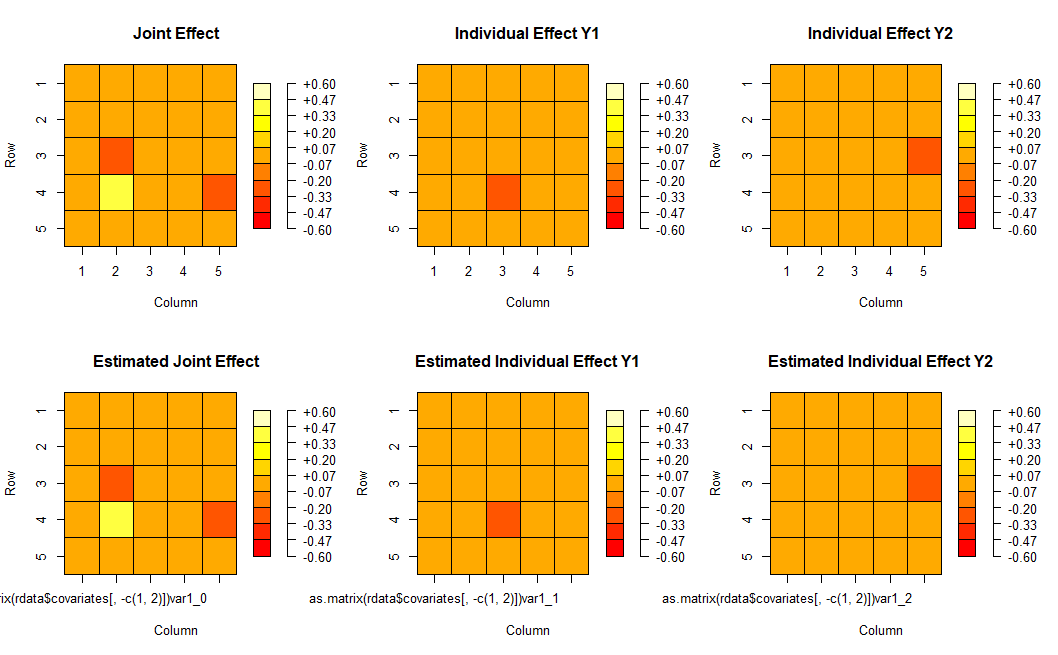
\includegraphics[width = \linewidth]{figures/2_VisRvarTrueEstPars}
		\caption{Illustration of the true and estimated Regression VAR parameters. For very large sample sizes, the traditional OLS method is successful. It would now be interesting to explore how regularization or model selection can help in higher dimension.}\label{fig:rvar_TrueEstimatedPars}
	\end{figure}
	
	\begin{figure}
		\centering
		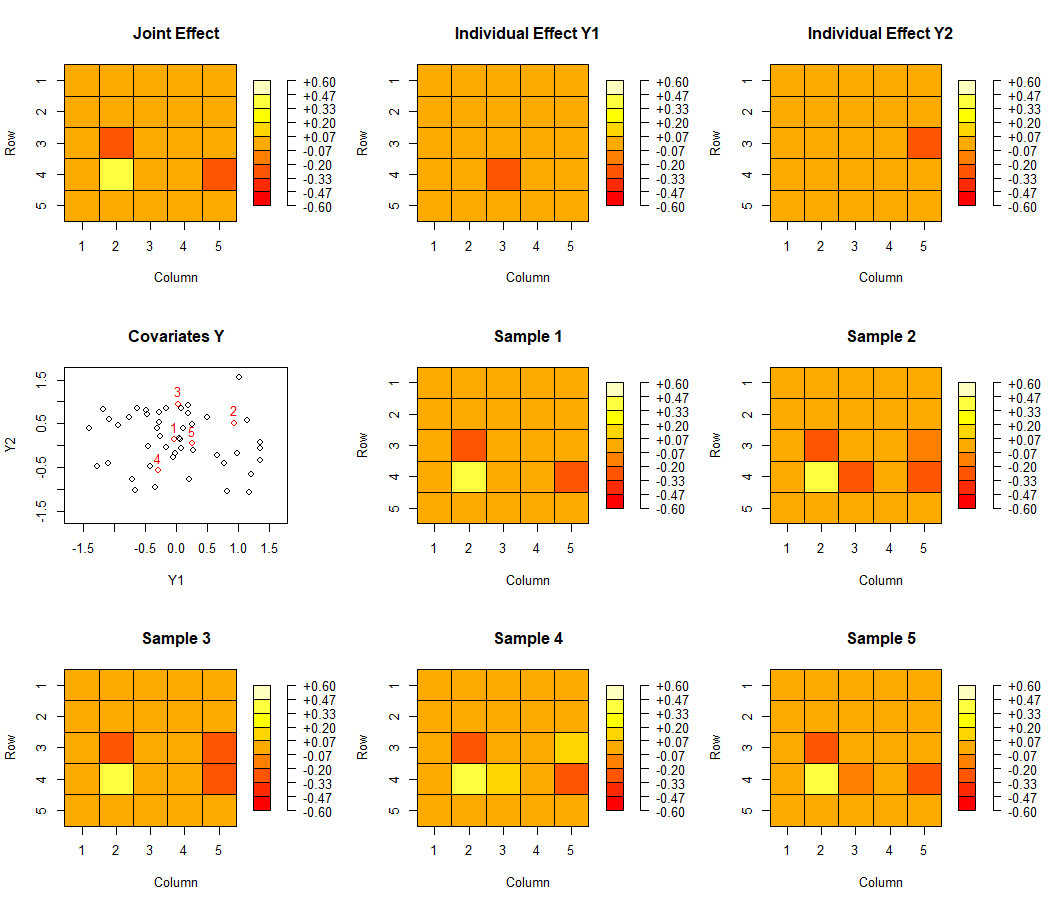
\includegraphics[width = \linewidth]{figures/1_VisParExample}
		\caption{Illustration of the Regression VAR framework with 2 covariate-dependent effects. Top-panels: visualization of the joint effects that are common across all subjects. We also visualize the effects that are individual to variables $Y_1$ and $Y_2$. Center-left panel: Visualization of the covariate information for $N = 50$ subjects. We highlight the covariate information of the first 5 subjects. Remaining panels: Visualization of the effects for the first 5 subjects. We observe that, as subject 1 has nearly zero for both $Y_1$ and $Y_2$, the effects are mostly just the joint effects. Subject 3 has a high $Y_2$ covariate, but low $Y_1$ covariate, and therefore its effects are a mixture of the joint and $Y_2$ effects. Subject 2 has large covariates for both $Y_1$ and $Y_2$, so its time series effects are a mixture of all.}\label{fig:rvarCoeffsExample}
	\end{figure}
	
	
	\item For this same example, we performed a traditional LS fitting, to see if we could successfully recover the common/individual structure of the time series. As we see in Figure \ref{fig:rvar_TrueEstimatedPars}, our estimation for very large sample sizes is successful.
	

	
	
\end{itemize}

\newpage

\section{Fitting the RVAR Model with LASSO Penalty}\label{section:rvar}


In this section, we describe the fitting of the RVAR model of the form \eqref{eq:rvar}, with 1-lag relationships, \textit{i.e.} $q = 1$. Assuming that, for each individual $k=1,...,N$, we can capture the VAR relationships in matrix form as:
{\footnotesize
\begin{equation*}
	\underbrace{\begin{bmatrix} 
		(X_{T_k}^k)^{'} \\ (X_{T_k-1}^k)^{'} \\ \vdots \\ (X_{2}^k)^{'}
	\end{bmatrix}}_{\Zb^{k}} = 
	\underbrace{\begin{bmatrix} 
		(X_{T_k-1}^{k})^{'}  & Y_{k1} (X_{T_k-1}^{k})^{'} &  Y_{k2} (X_{T_k-1}^{k})^{'} & \ldots & Y_{kp} (X_{T_k-1}^{k})^{'} \\
		(X_{T_k-2}^{k})^{'}  & Y_{k1} (X_{T_k-2}^{k})^{'} &  Y_{k2} (X_{T_k-2}^{k})^{'} & \ldots & Y_{kp} (X_{T_k-2}^{k})^{'} \\
		 \vdots      &     \vdots      & \ddots & \vdots 		  \\
		(X_{1}^{k})^{'}  & Y_{k1} (X_{1}^{k})^{'} &  Y_{k2} (X_{1}^{k})^{'} & \ldots & Y_{kp} (X_{1}^{k})^{'} \\
	\end{bmatrix}}_{\Wb^k} 
	\underbrace{\begin{bmatrix}
		\Psi_{0}^{'} \\ \Psi_{1}^{'} \\ \vdots \\ \Psi_{p}^{'}
	\end{bmatrix}}_{\Psi} +  
	\underbrace{\begin{bmatrix} 
		(\varepsilon_T^{k})^{'} \\ (\varepsilon_{T-1}^{k})^{'} \\ \vdots \\ (\varepsilon_{T-q+1}^{k})^{'}
	\end{bmatrix}}_{\Eb^{k}}.
\end{equation*}
}%
This can be simplified to matrix form as
\begin{equation}\label{eq:rvar_kmat}
	\Zb^{k} = \Wb^{k} \bPsi + \Eb^{k}
\end{equation}
The equation \eqref{eq:rvar_kmat} represents the VAR relationships for individual $k$. Then, we can model the behavior for all individuals via the equation
\begin{equation*}
	%\underbrace{\begin{bmatrix}  \Zb^1 \\ \Zb^2 \\ \vdots \\  \Zb^k \\ \vdots \\ \Zb^N \end{bmatrix}}_{\Zb} = 
	\underbrace{\begin{bmatrix}  \Zb^1 \\ \Zb^2  \\ \vdots \\ \Zb^N \end{bmatrix}}_{\Zb} = 
	%\underbrace{\begin{bmatrix}  \Wb^1 \\ \Wb^2 \\ \vdots \\  \Wb^k \\ \vdots \\ \Wb^N \end{bmatrix}}_{\Wb}  
	\underbrace{\begin{bmatrix}  \Wb^1 \\ \Wb^2  \\ \vdots \\ \Wb^N \end{bmatrix}}_{\Wb}  
	\bPsi + 
	%\underbrace{\begin{bmatrix}  \Eb^1 \\ \Eb^2 \\ \vdots \\  \Eb^k \\ \vdots \\ \Eb^N \end{bmatrix}}_{\Eb} 
	\underbrace{\begin{bmatrix}  \Eb^1 \\ \Eb^2 \\ \vdots \\ \Eb^N \end{bmatrix}}_{\Eb} 
\end{equation*}
We can finally summarize the VAR equation model for all individuals simultaneously with the reduced matrix equation:
\begin{equation}\label{eq:rvar_mat}
	\Zb = \Wb \bPsi + \bE.
\end{equation}
To solve for the parameter $\bPsi\in\bbR^{d (p+1) \times d}$, we propose performing the following optimization,
\begin{equation}\label{eq:rvar_matreg_lasso}
	\bhat\bPsi := \argmin_{\bPsi\in \bbR^{d (p+1) \times d}} \vertiii{ \Zb - \Wb \bPsi }_{F}^2 + \lambda_1 \vertiii{\Psi_{0}}_1 +  \lambda_2 \vertiii{[\Psi_1 \, \Psi_2 \, \ldots \, \Psi_p]}_1,
\end{equation}
where the hyperparameter $\lambda_1$ serves to penalize the common structure of all VAR models, and $\lambda_2$ penalizes the $Y$ covariate dependent portion of the model. We can interpret \eqref{eq:rvar_matreg_lasso} as a matrix regression problem. To solve the optimization problem \eqref{eq:rvar_matreg_lasso}, we use the \texttt{glmnet} package, which allows for solving matrix regression problems directly. The \texttt{glmnet} implementation  solves the problem by reducing the matrix regression problem to solving the regression problems of their individual columns.  
\begin{equation*}
	\bhat\bPsi^{\ell}(\lambda_1,\lambda_2) = \argmin_{\bPsi^{(\ell)} \in \bbR^{d (p+1)}} \vertiii{ \Zb_{\cdot \ell} - \Wb \bPsi^{(\ell)} }_{F}^2 + \lambda_1 \|{[\bPsi^{(\ell)}]_{1:d}}\|_1 +  \lambda_2 \|{[\bPsi^{(\ell)}]_{(d+1):(dp)}}\|_1.
\end{equation*}
Finally, we set the estimated parameter $\bhat\bPsi(\lambda_1,\lambda_2) := \left[\bhat\bPsi^{1}\, \bhat\bPsi^{2}\,\ldots \, \bhat\bPsi^{d}\right](\lambda_1,\lambda_2)\in\bbR^{d(p+1)\times d}$. Figure \ref{fig:rvar_TrueEstimatedPars} in the previous section was derived with $\lambda_1 = \lambda_2 = 0$.

The current implementation only allows for a single lagged relationship, \textit{i.e.} $q = 1$. We aim to create a more general implementation with lag $q> 1$ in the future.

\section{Fitting RUSEM}


The implementation of the RVAR model described in Section \ref{section:rvar} is simply a generalization of the optimization problem considered in the \citet{fisher2022penalized}. Notice that the RVAR focuses the estimation on the lagged effects $\bPsi$. For the GIMME model, we are also interested in recovering contemporaneous effects. The GIMME model cannot easily be extended to the regression setting. Therefore, we need to explore a different procedure for recovering the USEM structure in the regression setting. This will require thought and research...

I explored the original GIMME reference \citet{gates2012group}, which points towards the modification index described in \citet{sorbom1989model}. I am still trying to understand how the GIMME adapts the estimation of USEM described in \citet{sorbom1989model} to scenarios with time dependence. This will be the next task.











\bibliographystyle{apalike}
\bibliography{ref}


\end{document}
